\clearpage
\section{动画角色的方向光阴影}

固定相机与一块地面，让同一个角色反复播放待机动作。场景面板为 $600\times385$，只有一盏投影的方向光。开启“角色阴影”后，地面上能分辨出身体和手臂的轮廓。新增开销来自按灯的方向画一次当前姿势，并在计算直接光时查询这张图。

\begin{center}
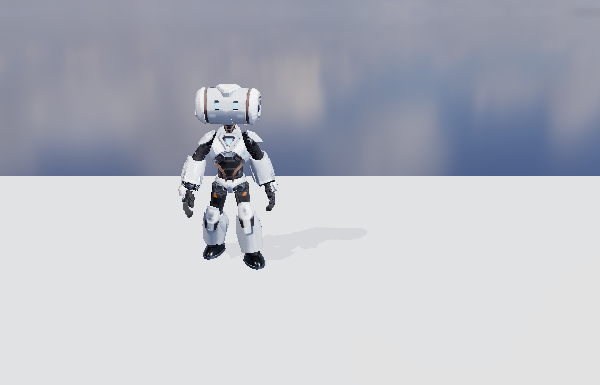
\includegraphics[width=.48\linewidth]{../../../output/validation/animated-shadows/left-on.png}\hfill
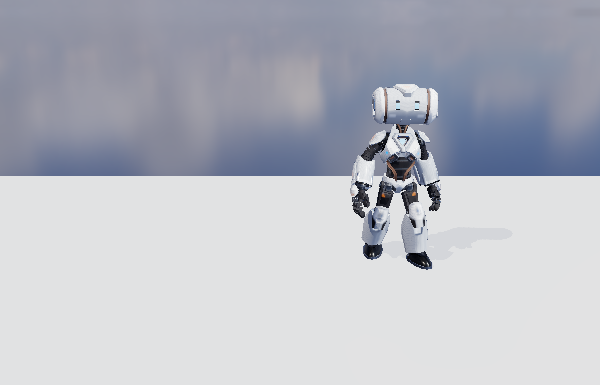
\includegraphics[width=.48\linewidth]{../../../output/validation/animated-shadows/right-on.png}\\
{\small 同一台相机下，角色和地面阴影一同向右移动。两张图均为 Vulkan 面板实拍。}
\end{center}

在 NVIDIA GeForce RTX 5070 Ti Laptop GPU 上运行 Debug 构建，把相同设置的第 8 帧交给 RenderDoc 1.47 回放。每份帧先预热一次，再重复读取 11 次事件时间，表中取中位数。事件总和包括本帧的绘制与计算，不包含呈现、队列空闲时间或 CPU 等待。

{\smalltable\noindent\begin{tabularx}{\linewidth}{@{}Xrr@{}}\toprule
一帧中的工作 & 关闭 & $512\times512$\\\midrule
GPU 绘制与计算事件总和 & 0.202\,ms & 0.239\,ms\\
其中：计算直接光 & 0.016\,ms & 0.019\,ms\\
从灯的位置绘制角色七个部件 & 0 & 0.027\,ms\\
保存这一盏灯的角色深度 & 0 & 0.005\,ms\\\bottomrule
\end{tabularx}\par}

CPU 另在未截帧的编辑器里计时。按关闭、开启、开启、关闭运行四次，每次连续播放 90 帧，去掉前 20 帧，每种设置保留 140 个读数。\texttt{Rasterize lighting surfaces} 包含相机表面、角色阴影的命令录制以及这段调用中的驱动等待：关闭时中位数为 1.415\,ms，开启后为 2.083\,ms。在同一台机器上，从仓库根目录运行 \path{tests/check_animated_shadows.py} 并带 \texttt{--cpu-only} 可重复测量。逐帧读数见 \path{output/validation/animated-shadows/cpu.json}。

每盏灯保存一张 $512^2$ 的单精度深度图，像素正好占 1\,MiB，另外保存矩阵和索引。不同方向的灯依次共用光源视角的绘制目标。现在仍用现有表面着色器写入颜色、法线和深度，最终只用其中的深度。下一次可以单独测量只写深度并保留材质镂空裁剪的画法。场景里相距很远的角色会共享整张图，一个像素覆盖的世界范围随之变大，近处角色的轮廓也会变粗，这种分布另需单独测试。点光源的动态遮挡及透明材质的透光都未纳入本次测量。

截帧入口为 \path{tests/check_animated_shadows.py}。两个 \texttt{moving} 对照的 JSON 分别保留本地 RDC 路径、二进制与捕获文件的 SHA-256、GPU 逐次读数、事件编号。图中的角色由 Juan Linietsky 与 Fernando Miguel Calabró 为 Godot 第三人称样例创作，使用 CC BY 3.0。Redflag 的导入说明和版本见 \path{RedflagForge/assets/game/station/crew/README.md}。
